\documentclass[12pt,a4paper]{article}
\usepackage{ctex}
\usepackage{graphicx}
\usepackage{geometry}
\usepackage{array}
\usepackage{amssymb}
\usepackage{setspace}
\usepackage{xeCJK}
\usepackage{indentfirst}
\usepackage{amsmath}
\usepackage{amsthm}
\usepackage{float}
\usepackage{subfigure}
\usepackage{booktabs}
\usepackage{multirow}
\usepackage{caption}
\usepackage{listings}
\usepackage{xcolor}
\usepackage{matlab-prettifier}
\usepackage{enumitem}
\captionsetup[table]{position=bottom}

% 页边距
\geometry{left=2.5cm,right=2.5cm,top=2.5cm,bottom=2.5cm}
% 默认宋体小四
\setCJKmainfont[BoldFont=SimHei]{SimSun}
\zihao{-4}
\linespread{1.25}

\lstdefinestyle{Matlab-boxed}{
  style=Matlab-editor,
  frame=single,
  framerule=0.6pt,
  rulecolor=\color{black},
  framesep=6pt,
  backgroundcolor=\color{black!2},
  basicstyle=\footnotesize\ttfamily,
}

\begin{document}
% 实验名称（小二黑体、居中）
\begin{center}
  {\zihao{2}\heiti 迈克尔逊干涉仪测光波波长}
\end{center}
% 年级 专业 姓名 座位号（宋体小四、居中、段前后 0.5 行）
\vspace{0.1\baselineskip}
\begin{center}
  （\textbf{年级}\ \underline{2024 级}\quad \textbf{专业}\ \underline{x} \quad \textbf{姓名}\ \underline{Pinco Li} \quad \textbf{座位号} \ \underline{5}）
\end{center}
\vspace{0.1\baselineskip}

\section{实验目的}

\begin{enumerate}
  \item 了解迈克尔逊干涉仪的基本结构、工作原理及其调节方法
  \item 观察等倾干涉和等厚干涉现象，理解两种干涉类型的形成条件及特征
  \item 学习利用干涉条纹的移动来精密测量光波波长
  \item 掌握光程差的概念及其在干涉测量中的应用
\end{enumerate}

\section{实验仪器}

\begin{figure}[H]
\centering
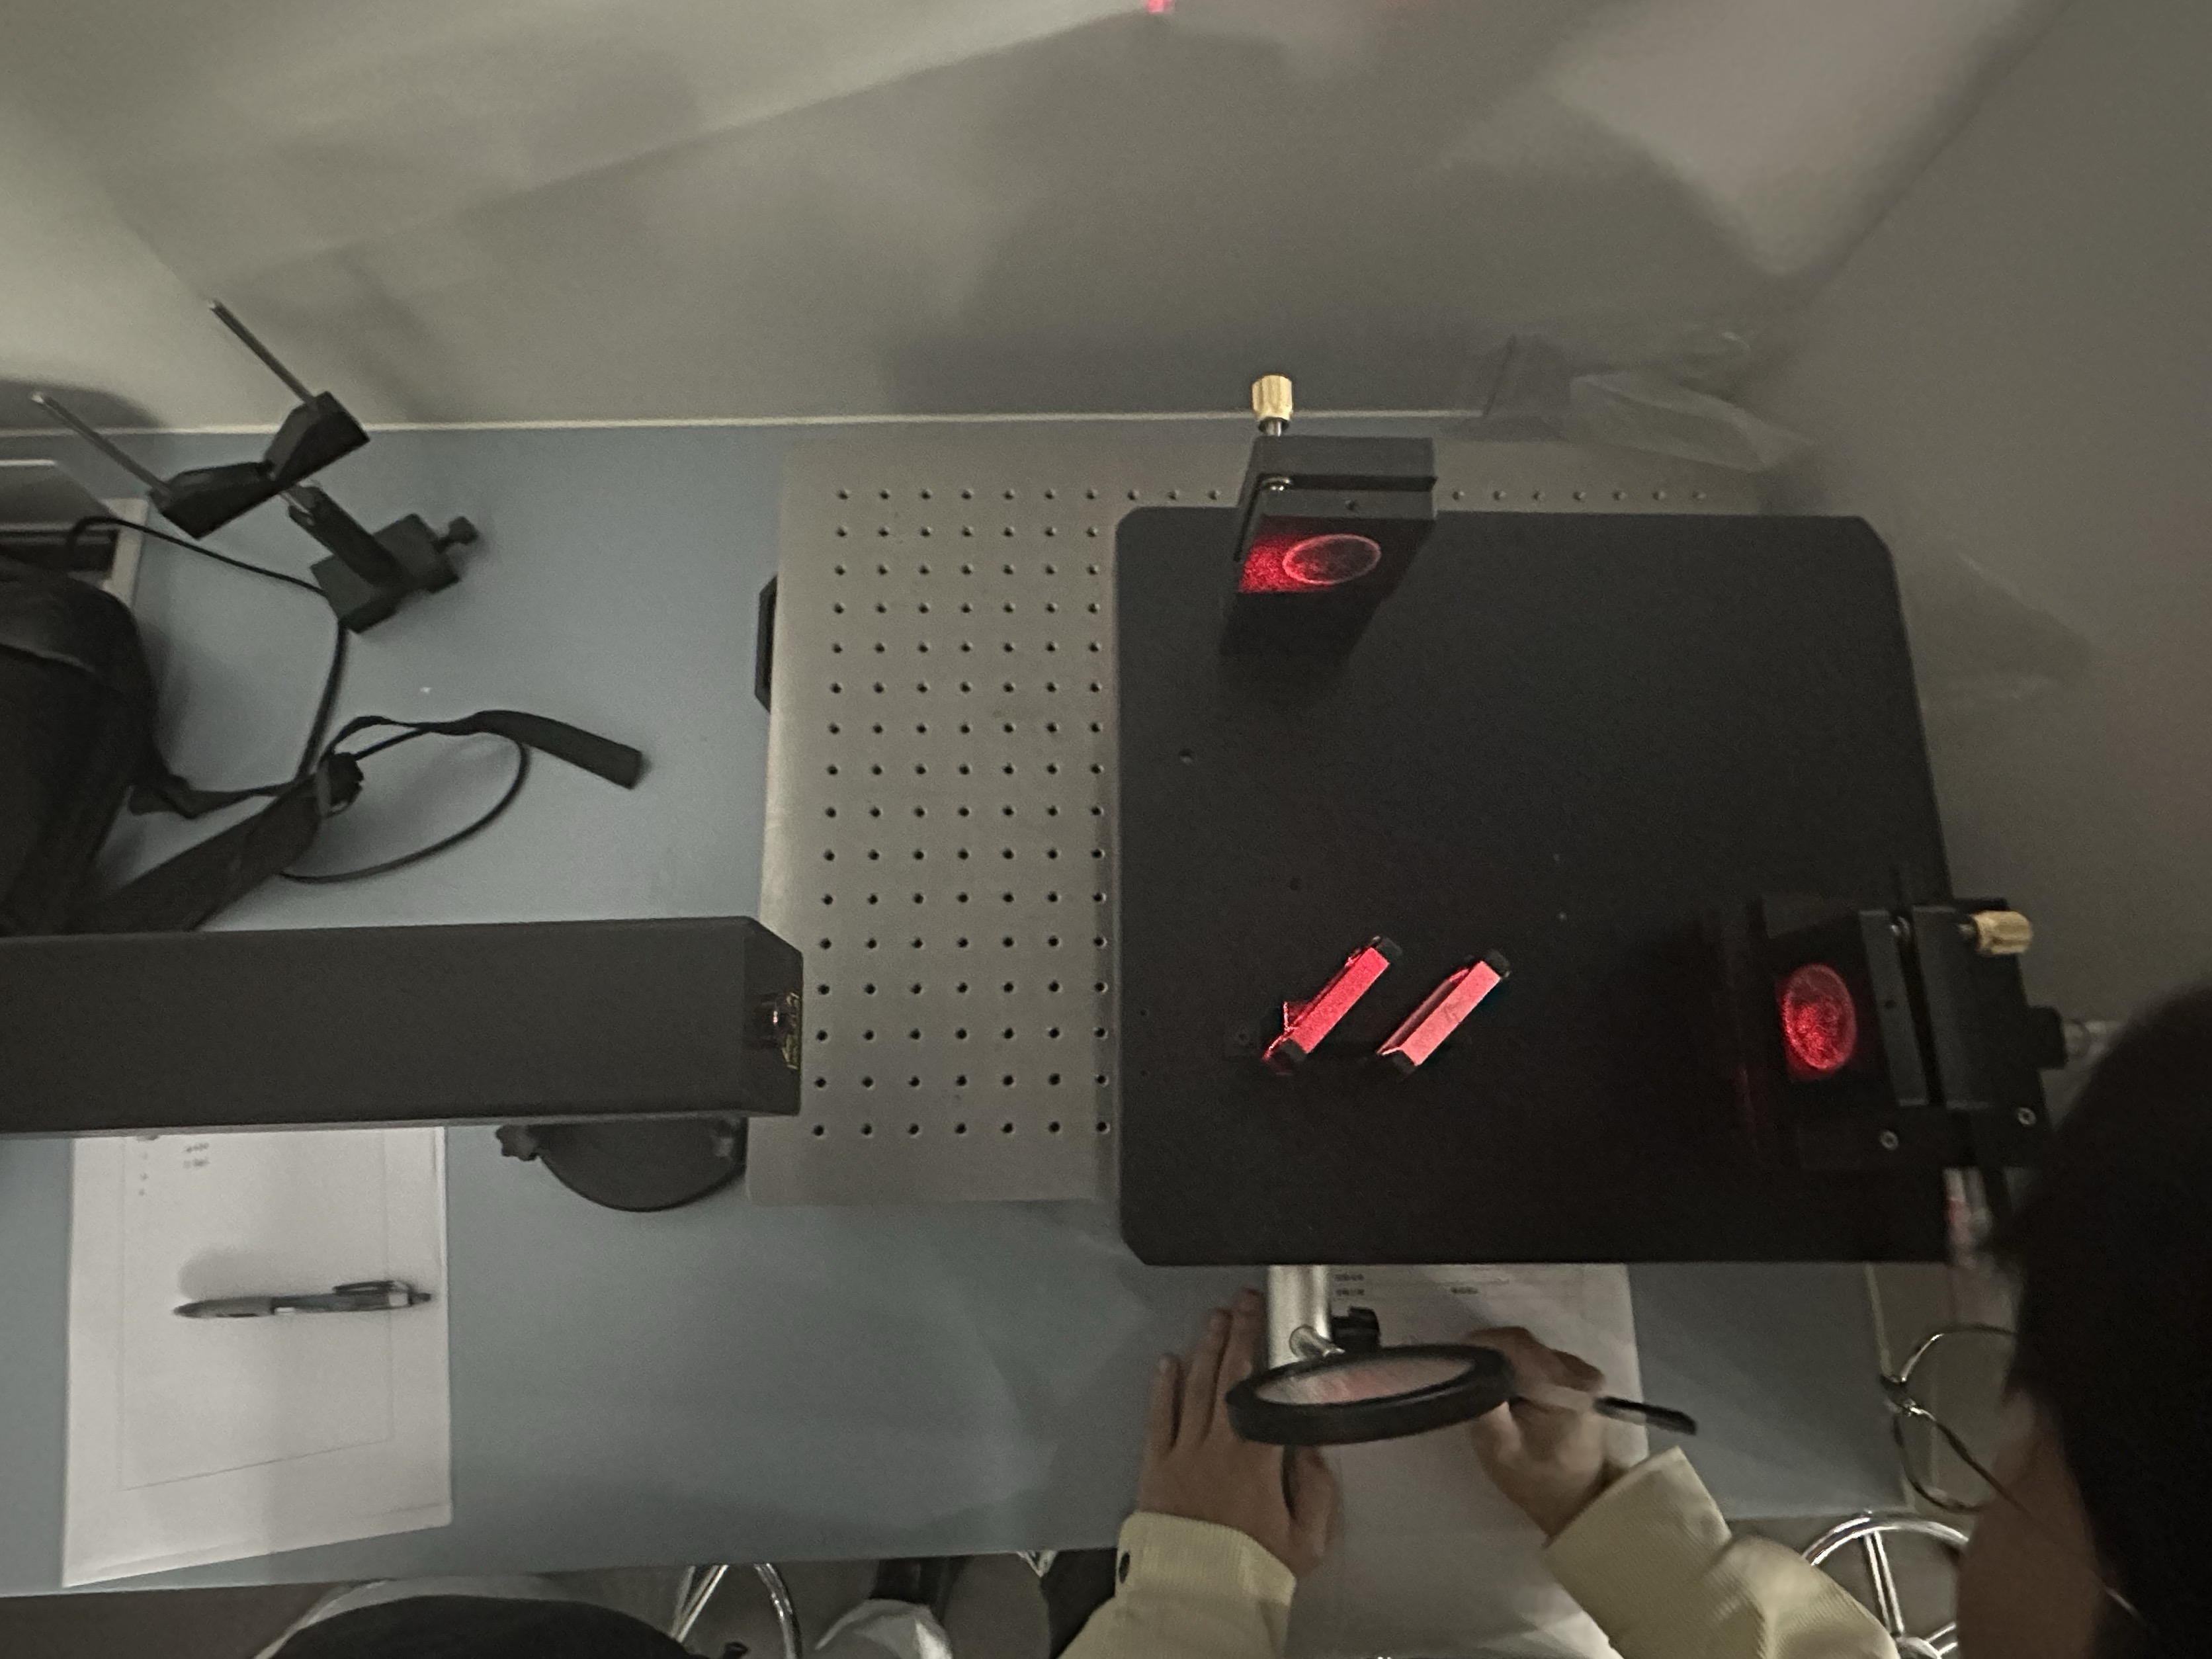
\includegraphics[width=0.7\textwidth]{assets/实验仪器.jpg}
\caption{实验仪器}
\label{fig:experiments}
\end{figure}

\begin{enumerate}
    \item 迈克尔逊干涉仪主体（含分光器 $G_1$、补偿器 $G_2$、动镜 $M_1$、定镜 $M_2$）
    \item He-Ne 激光器（波长标称值 632.8 nm）
    \item 扩束镜
    \item 观察屏（毛玻璃）
    \item 测微螺旋（读数精度 0.01 mm）
\end{enumerate}

\section{实验原理}

\subsection{迈克尔逊干涉仪的光路结构}

迈克尔逊干涉仪是1881年由美国物理学家迈克尔逊（A. A. Michelson）设计制造的精密光学仪器，它利用分振幅法产生双光束干涉。该仪器在光学测量、精密检测和基础物理研究中有着广泛应用，迈克尔逊本人也因使用该仪器进行的以太漂移实验而获得1907年诺贝尔物理学奖。

从光源 $S$ 发出的光束经扩束后到达分光器 $G_1$，$G_1$ 是一块在对角面上镀有半反射膜的平行平面玻璃板。入射光在 $G_1$ 的半反射面上被分成两束振幅近似相等的相干光：一束光被反射至动镜 $M_1$，经 $M_1$ 反射后再次回到 $G_1$，透过半反射面到达观察器；另一束光透过 $G_1$ 到达定镜 $M_2$，经 $M_2$ 反射后回到 $G_1$，在半反射面上反射后同样到达观察器。这两束相干光在观察器处叠加产生干涉现象。

在这一光路中存在一个光程补偿问题：第一束光在玻璃介质中传播了三次（入射时透过玻璃基底，反射回来时在玻璃中传播两次），而第二束光仅在玻璃中传播一次。为了使两束光在玻璃介质中的光程相等，在第二束光的光路中插入一块与 $G_1$ 完全相同的平行平面玻璃板 $G_2$，称为补偿器。加入补偿器后，两束光在玻璃介质中的光程完全相同，从而保证了在使用白光照明时也能观察到清晰的干涉条纹。

\subsection{等倾干涉与等厚干涉}

根据两个反射镜 $M_1$ 和 $M_2$ 的相对位置关系，迈克尔逊干涉仪可以产生两种不同类型的干涉图样。

\textbf{等倾干涉：}当动镜 $M_1$ 与定镜 $M_2$ 严格平行时，可以将 $M_2$ 看作 $M_1$ 在分光器中的虚像 $M_2'$。此时 $M_1$ 与 $M_2'$ 形成一个平行的空气薄层，厚度记为 $d$。对于从光源不同角度入射的光线，尽管入射点不同，但只要入射角 $i$ 相同，它们在两个反射面之间产生的光程差就相同，因而干涉加强或减弱的条件也相同。这种相同倾角的光线经透镜会聚后在焦平面上形成同一条干涉条纹，这类干涉称为等倾干涉。等倾干涉的特征是形成一系列同心圆环，圆环的级次从中心向外依次降低。

\textbf{等厚干涉：}当动镜 $M_1$ 与定镜 $M_2$ 之间存在微小夹角 $\alpha$ 时，$M_1$ 与虚像 $M_2'$ 构成一个楔形空气薄层。在垂直入射的情况下，光程差仅取决于该点处空气层的厚度。厚度相同的位置产生相同级次的干涉条纹，因此称为等厚干涉。等厚干涉的特征是形成一系列近似平行的直条纹，条纹的取向垂直于两镜交线的方向。

在实际观察中，可以通过调节动镜背后的微调螺钉来改变 $M_1$ 与 $M_2$ 的相对倾斜程度，从而在等倾干涉和等厚干涉之间切换，甚至观察到两者的过渡形态。

\subsection{光程差与干涉条件}

\begin{figure}[H]
\centering
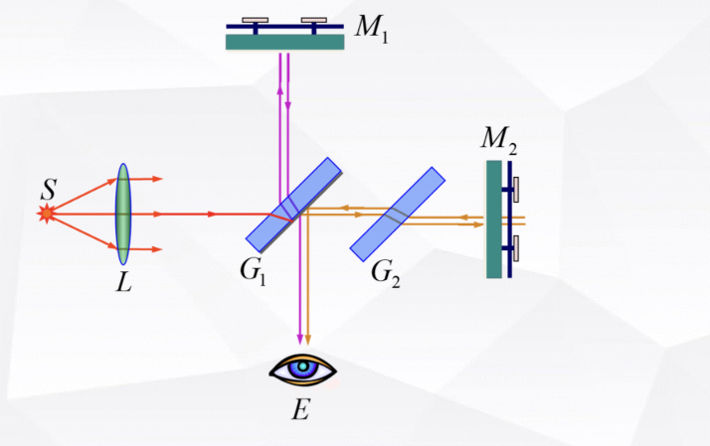
\includegraphics[width=0.6\textwidth]{assets/光路图.png}
\caption{光路原理图}
\label{fig:lightway}
\end{figure}

对于等倾干涉的情形，设空气层厚度为 $d$，光线以入射角 $i$ 入射。光线在空气层中往返一次的光程为 $\overline{AB} + \overline{BC} = 2d\cos i$，另一束光的光程为 $\overline{AD}$。由几何关系可知，两束光的光程差为
\begin{equation}
\delta = 2d \cos i.
\end{equation}

当光程差满足
\begin{equation}
\delta = 2d \cos i = k\lambda, \quad k \in \mathbb{Z}
\end{equation}
时，两束光发生相长干涉，产生亮条纹（干涉极大）。其中 $k$ 称为干涉级次，$\lambda$ 为光波波长。

对于中心点，光线垂直入射，即 $i = 0$，此时 $\cos i = 1$，光程差为
\begin{equation}
\delta = 2d = k\lambda.
\end{equation}

当动镜移动一段距离 $\Delta d$ 时，光程差的变化量为 $\Delta \delta = 2\Delta d$。设在此过程中观察到条纹数的变化量为 $N$（即有 $N$ 个条纹从中心涌出或缩入），则干涉级次的变化量为 $\Delta k = N$。由于 $\Delta \delta = \Delta k \cdot \lambda$，可得
\begin{equation}
2\Delta d = N\lambda,
\end{equation}
从而可以通过测量动镜位移 $\Delta d$ 和对应的条纹数变化 $N$ 来计算光波波长：
\begin{equation}
\lambda = \frac{2\Delta d}{N}.
\label{eq:wavelength}
\end{equation}

这一关系式是利用迈克尔逊干涉仪测量光波波长的理论基础。通过精确测量动镜的位移量和对应的干涉条纹数，可以高精度地测定光波波长。

\section{实验步骤}

\subsection{仪器调整与准备}

实验开始前，首先需要正确认识迈克尔逊干涉仪各部件的位置和功能。将激光器、分光器、动镜、定镜和观察屏按照光路要求粗略摆放好。将动镜的测微螺旋调至中间位置（约 25 mm 处），以便后续向两个方向调节时都有足够的行程。

为了观察到清晰的干涉条纹，必须使两束反射光尽可能完全重合。首先移开激光器镜头前的扩束镜，使激光以较细的光束入射。调节动镜（激光器正对的反射镜）背面的两个微调螺钉，使其反射光斑与入射光斑在分光器附近尽可能重合。这一步骤的判据是：从侧面观察时，两个光斑应当重叠或非常接近。

接下来调节定镜（观测者正对的反射镜）背面的微调螺钉，使其反射光点与动镜的反射光点在空间中重合。这一步骤较为关键，需要仔细观察两个光点的位置，通过微调螺钉使它们在水平和竖直方向上都对齐。

\subsection{干涉条纹的形成与优化}

完成粗调后，一手轻轻固定激光器以防止其大幅摆动，另一手将扩束镜插入光路中。扩束后的光束会在两个反射镜上形成较大的光斑，此时在观察屏（毛玻璃）上应当能够看到干涉条纹。如果条纹不明显或完全看不到，说明两束光的平行度不够好，需要继续微调反射镜背后的螺钉。

\begin{figure}[H]
\centering
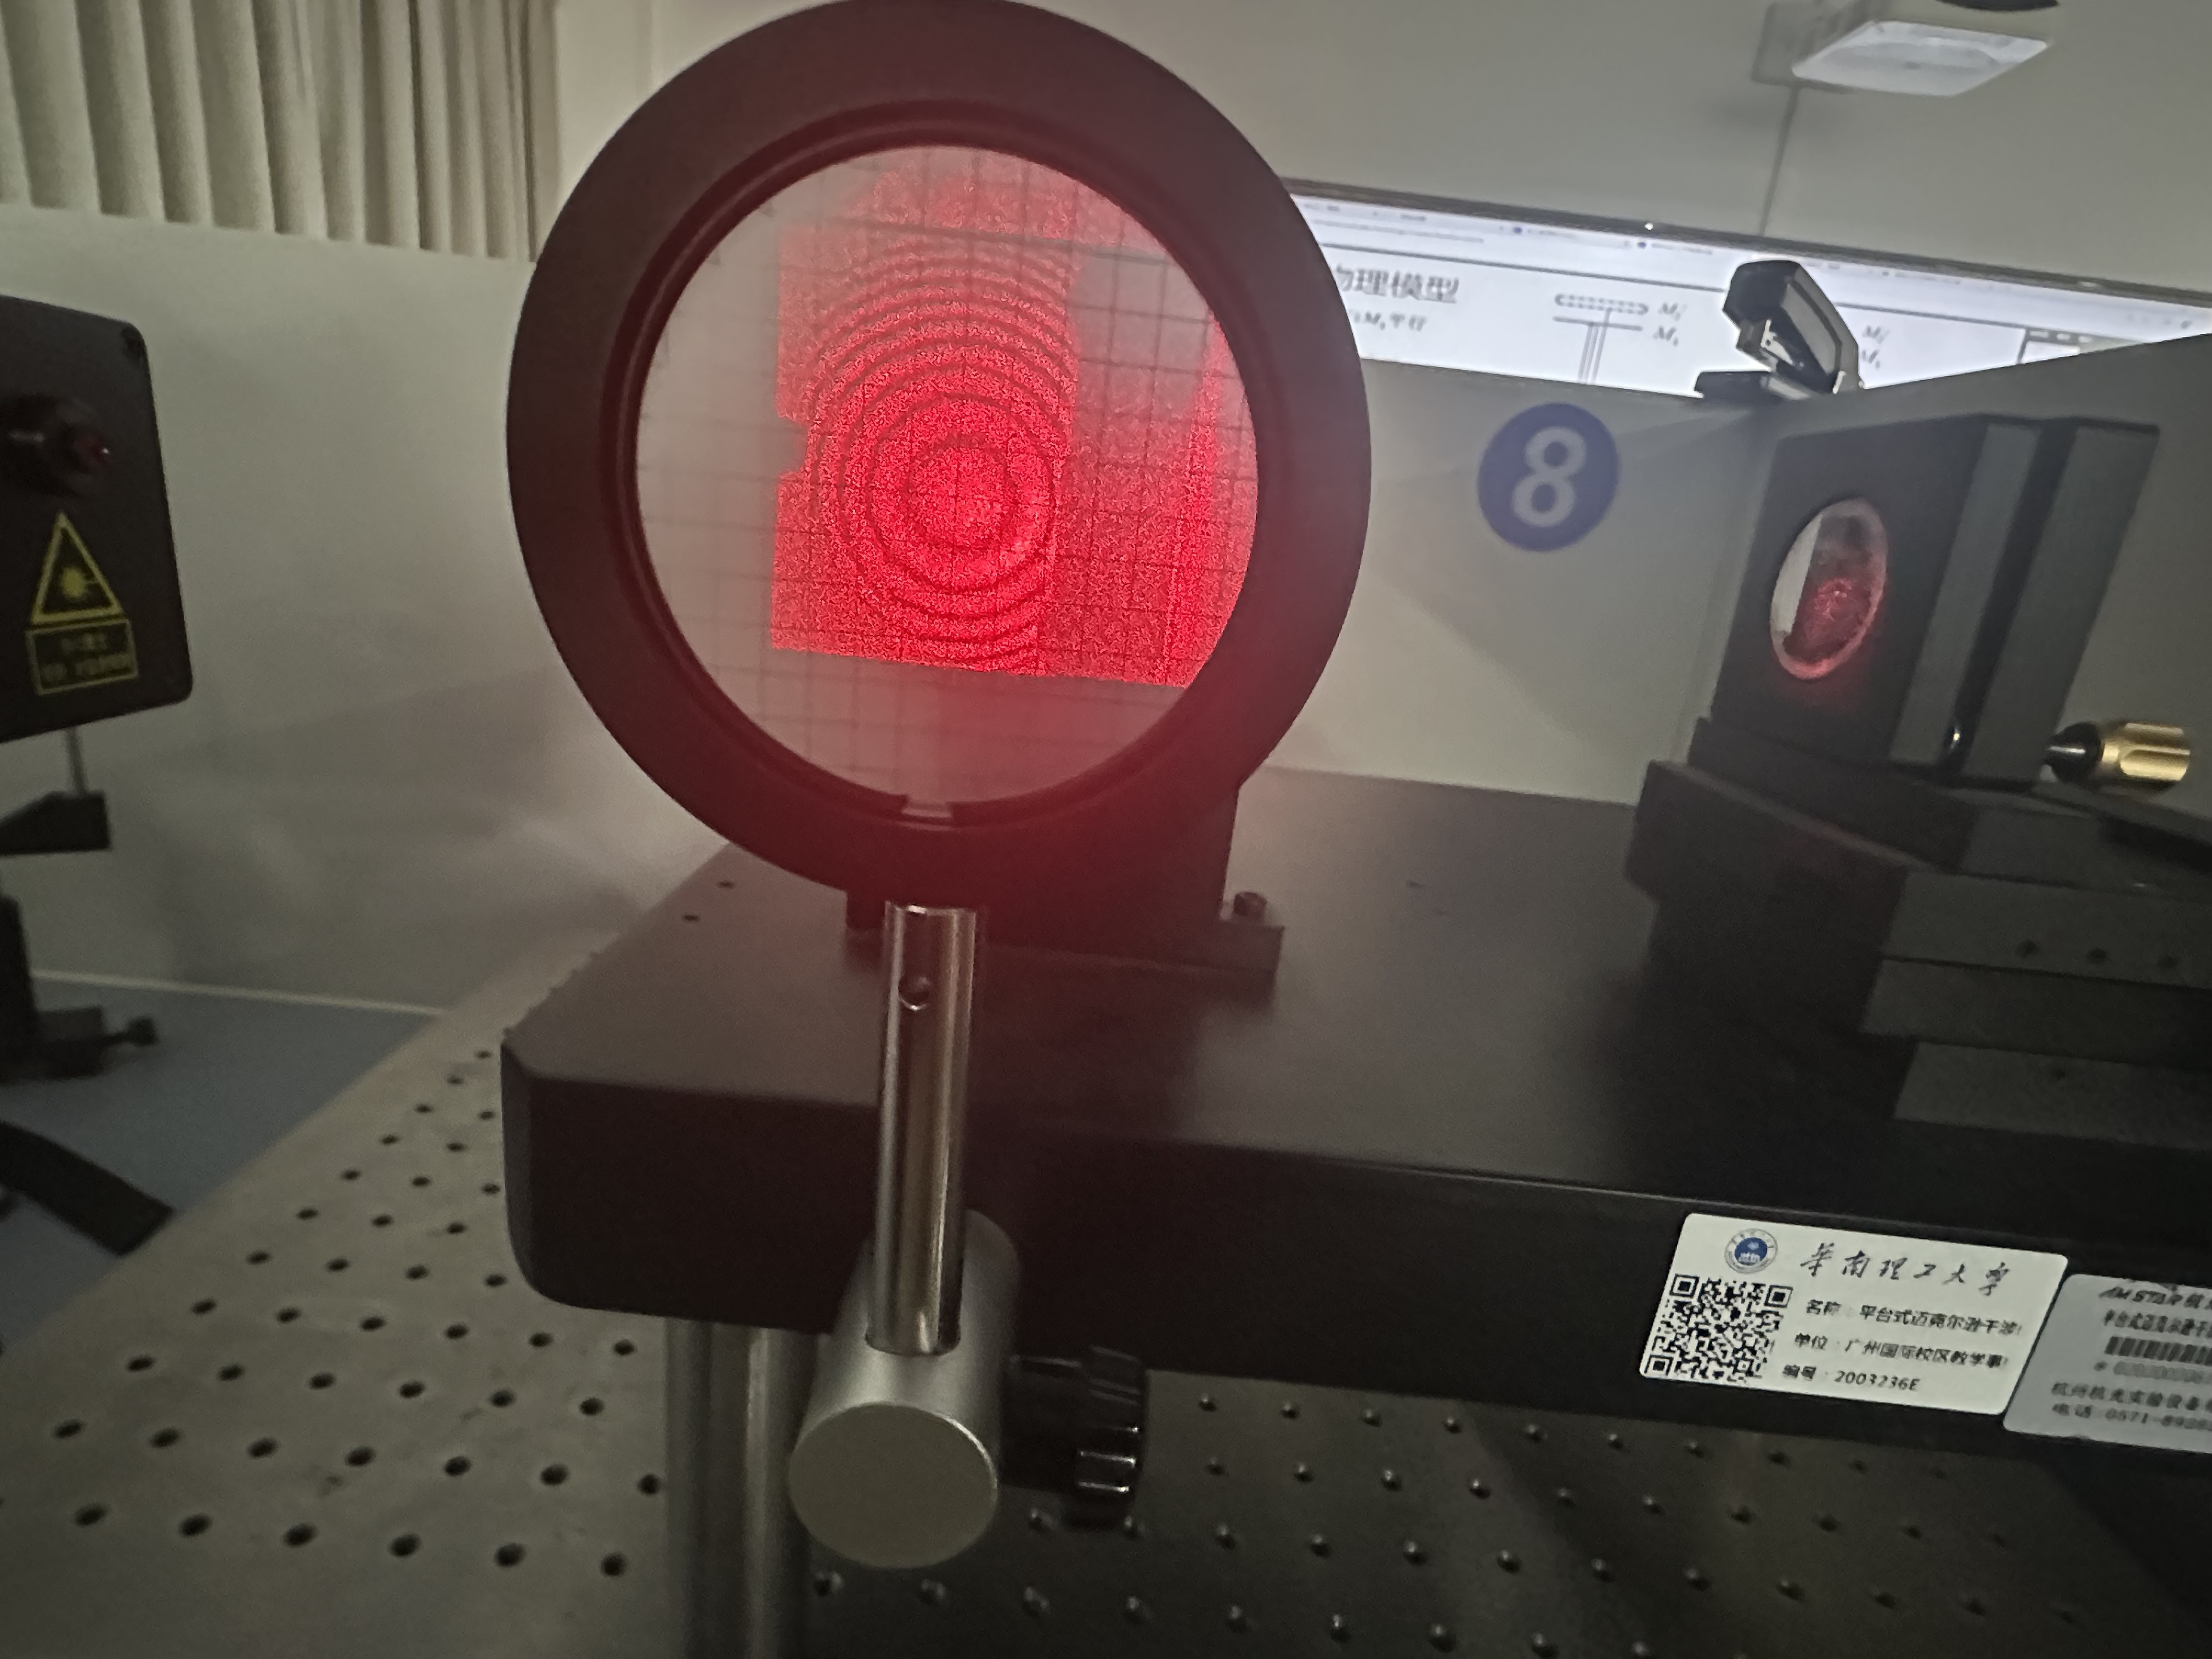
\includegraphics[width=0.75\textwidth]{assets/干涉条纹实拍.jpg}
\caption{干涉条纹示意图}
\label{fig:light-display}
\end{figure}

观察条纹的形状和位置。对于等倾干涉，条纹应呈现为一系列同心圆环；对于等厚干涉，条纹应为一组近似平行的直线。通过调节螺钉，可以改变两镜之间的夹角，从而在两种干涉类型之间切换。为了进行波长测量，需要调整至等倾干涉状态，并使圆环的中心尽可能位于视场的中心位置。若条纹中心偏离视场中心，可通过微调螺钉将其移至中心。

\subsection{波长测量}

调整完毕后，开始进行波长测量。记录下测微螺旋的初始读数。缓慢旋转测微螺旋，使动镜沿光轴方向移动，同时注意观察毛玻璃上的干涉条纹变化。随着动镜的移动，干涉圆环会从中心涌出或向中心收缩。选择一个方向（例如动镜向远离分光器的方向移动，条纹从中心涌出），开始计数通过中心的条纹数。

为了提高测量精度，采用分段测量的方法。每当有 50 个条纹通过中心时，记录一次测微螺旋的读数。这样可以多次测量，既能减小计数误差，又能通过线性拟合的方法检验实验的系统性和可靠性。本实验共测量了 12 组数据，条纹数从 50 个累积到 600 个，对应的测微螺旋读数依次记录。

测量过程中应注意以下几点：旋转测微螺旋时动作要缓慢平稳，避免因振动导致条纹模糊；计数时要集中注意力，避免漏数或重复计数；每次读数时要等待系统稳定，确保读数准确；始终保持同一旋转方向，避免因螺旋的回程误差影响测量精度。

\section{数据记录与处理}

\subsection{原始数据}

本实验测量了在动镜连续移动过程中，干涉条纹数与测微螺旋读数之间的对应关系。初始读数为 5.000，每当有 50 个条纹通过视场中心时记录一次读数。原始数据如表~\ref{tab:raw_data} 所示。

\begin{table}[H]
\centering
\caption{干涉条纹数与测微螺旋读数}
\label{tab:raw_data}
\begin{tabular}{|c|c|c|c|}
\hline
\textbf{条纹数 $N$} & \textbf{读数} & \textbf{条纹数 $N$} & \textbf{读数} \\
\hline
0   & 5.000  & 300 & 14.482 \\
\hline
50  & 6.370  & 350 & 15.979 \\
\hline
100 & 7.763  & 400 & 17.475 \\
\hline
150 & 9.405  & 450 & 18.978 \\
\hline
200 & 11.378 & 500 & 20.538 \\
\hline
250 & 12.968 & 550 & 22.018 \\
\hline
&  & 600 & 23.510 \\
\hline
\end{tabular}
\end{table}

需要说明的是，测微螺旋的读数并非直接以毫米为单位，而是经过了刻度转换。根据仪器说明，读数与实际位移的转换系数为 0.01 mm/格，即每格读数对应 0.01 mm 的实际位移。

\subsection{数据处理与线性拟合}

将读数转换为实际位移量后，以条纹数 $N$ 为横坐标、动镜位移 $\Delta d$ 为纵坐标进行线性拟合。根据理论公式~(\ref{eq:wavelength})，位移与条纹数之间应满足线性关系
\begin{equation}
\Delta d = k \cdot N + b,
\end{equation}
其中斜率 $k = \lambda / 2$ 包含了波长信息，截距 $b$ 理论上应接近零。

采用最小二乘法对实验数据进行线性拟合，得到拟合参数如下：
\begin{itemize}
    \item 斜率：$k = 0.000313$ mm/条纹 $= 0.313$ $\mu$m/条纹
    \item 截距：$b = -0.001049$ mm $\approx -1.05$ $\mu$m
    \item 决定系数：$R^2 = 0.999097$
\end{itemize}

拟合结果的决定系数 $R^2$ 非常接近 1，表明实验数据与线性模型高度吻合，验证了理论预期的线性关系。如图~\ref{fig:fit} 所示，实验数据点几乎完全落在拟合直线上，表明实验过程系统性良好，随机误差较小。

\begin{figure}[H]
\centering
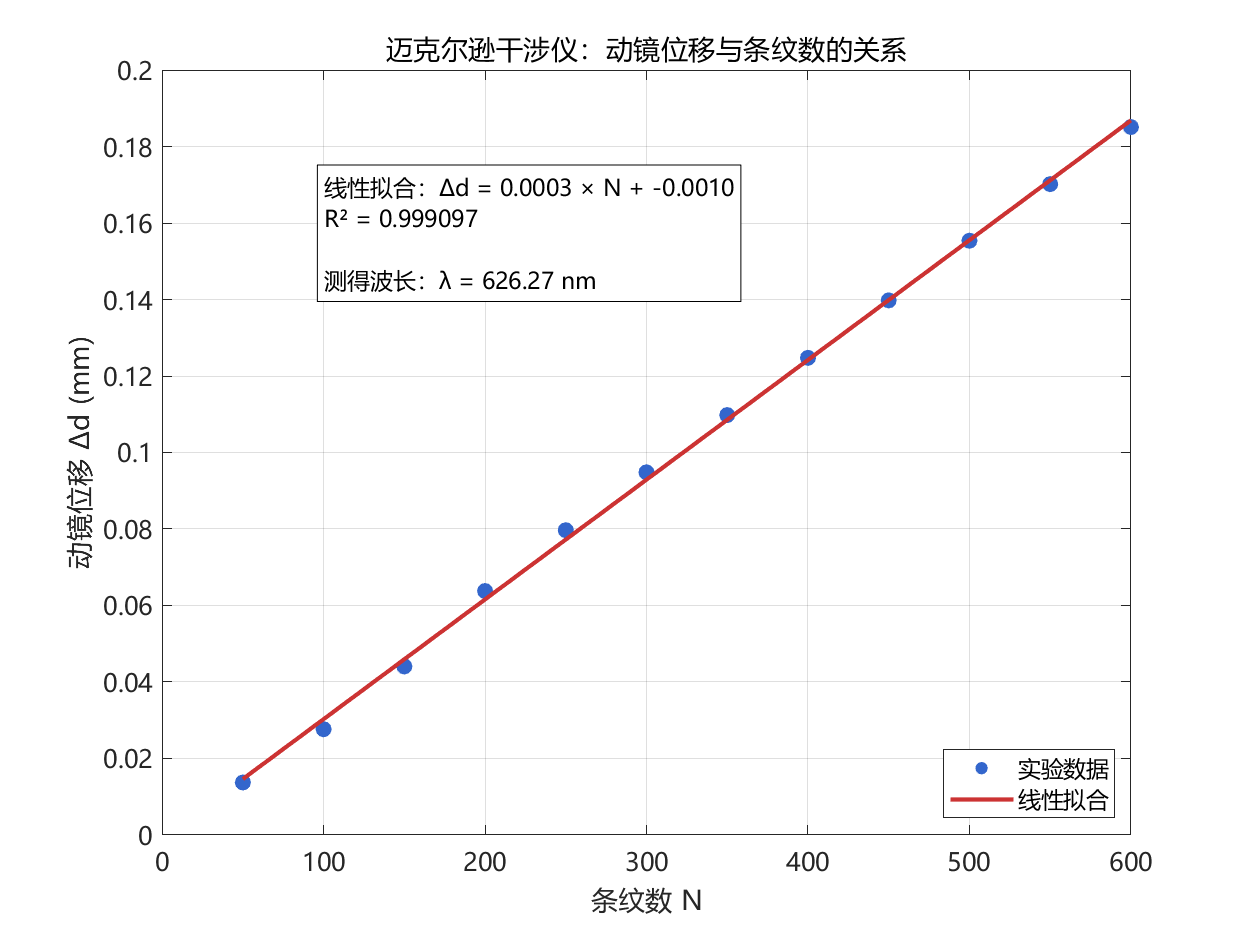
\includegraphics[width=0.75\textwidth]{assets/图1_位移条纹关系.png}
\caption{动镜位移与干涉条纹数的线性关系}
\label{fig:fit}
\end{figure}

截距 $b$ 的非零值（约 $-1.05$ $\mu$m）可能来源于初始读数的零点漂移或者测量起点处干涉条纹级次判断的微小偏差，但其绝对值远小于整个测量范围（约 0.185 mm），对最终结果的影响可以忽略。

\subsection{波长计算}

根据拟合得到的斜率 $k$ 和理论关系式 $\lambda = 2k$，可以计算出光波波长：
\begin{equation}
\lambda = 2 \times 0.000313 \text{ mm} = 0.000626 \text{ mm} = 626.27 \text{ nm}.
\end{equation}

为了评估结果的不确定度,可以利用线性拟合的统计方法。设残差标准差为 $s$，自变量的标准差为 $s_x$，则斜率的标准不确定度为
\begin{equation}
u(k) = \frac{s}{\sqrt{n-2} \cdot s_x},
\end{equation}
其中 $n = 12$ 为数据点数。经计算得到 $u(k) = 0.000003$ mm/条纹，对应波长的不确定度为
\begin{equation}
u(\lambda) = 2 u(k) = 5.95 \text{ nm}.
\end{equation}

因此，本实验测得的光波波长可表示为
\begin{equation}
\lambda = (626.3 \pm 6.0) \text{ nm} \quad (k=1).
\end{equation}

He-Ne 激光的标准波长为 632.8 nm。将测量结果与标准值比较，相对误差为
\begin{equation}
\delta = \frac{|626.27 - 632.8|}{632.8} \times 100\% = 1.03\%.
\end{equation}

这一结果表明，利用迈克尔逊干涉仪测量光波波长具有很高的精度，测量值与理论值符合良好。

\subsection{残差分析与波长分布}

为了进一步检验实验数据的质量，对拟合残差进行分析。残差定义为实验测量值与拟合值之差。如图~\ref{fig:residual} 上图所示，各数据点的残差在零线附近随机分布，无明显的系统趋势，表明线性模型能够很好地描述实验数据，不存在显著的系统性偏差。

此外，对每组数据（每 50 个条纹对应一组）分别计算波长，得到 12 个独立的波长测量值。这些测量值的平均值为 610.42 nm，标准差为 29.64 nm。如图~\ref{fig:residual} 下图所示，各组测量值在理论值附近分散，但总体趋势与理论值一致。需要注意的是，单组数据计算波长时由于条纹数较少，相对不确定度较大；而通过线性拟合综合利用所有数据点，能够显著提高测量精度。

\begin{figure}[H]
\centering
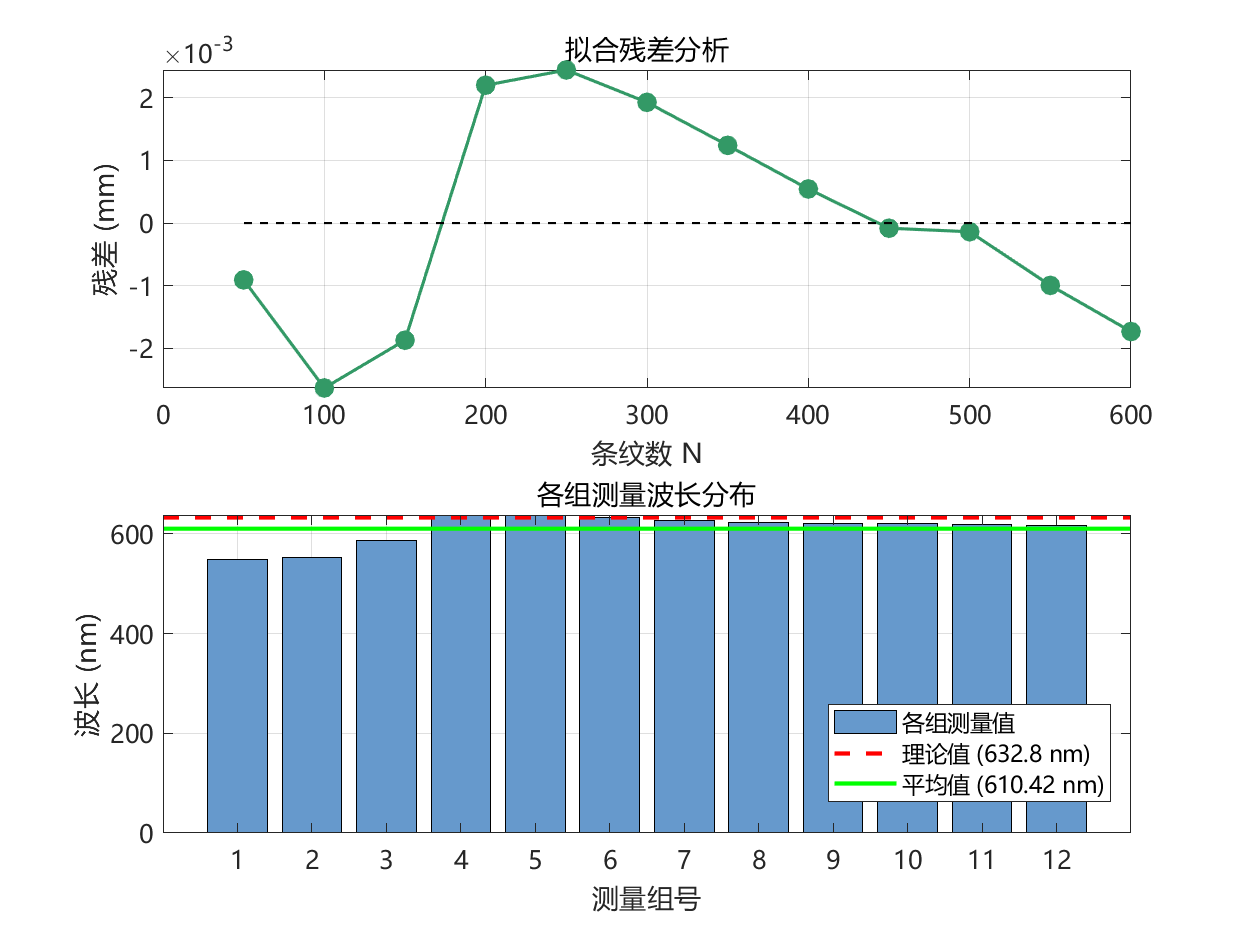
\includegraphics[width=0.85\textwidth]{assets/图2_残差与波长分布.png}
\caption{拟合残差分析（上）与各组波长测量值分布（下）}
\label{fig:residual}
\end{figure}

\section{干涉图样的模拟与分析}

为了更好地理解迈克尔逊干涉仪中两种干涉类型的形成机制及其图样特征，利用 MATLAB 对等倾干涉和等厚干涉进行了数值模拟。模拟基于光程差与相位差的关系，计算空间各点的光强分布，从而重现实验中观察到的干涉图样。

\subsection{等倾干涉模拟}

在等倾干涉的情形下，动镜 $M_1$ 与虚像 $M_2'$ 平行，形成厚度为 $d$ 的均匀空气层。对于入射角为 $i$ 的光线，光程差为 $\delta = 2d\cos i$。在小角度近似下，入射角 $i$ 与距光轴的距离 $r$ 成正比。因此，距光轴距离相同的点具有相同的光程差，干涉条纹呈现为同心圆环。

模拟中设空气层厚度 $d = 10$ $\mu$m，波长 $\lambda = 632.8$ nm。计算得到的光强分布如图~\ref{fig:equal_incline} 所示。左图为二维光强分布图，清晰地展示了同心圆环结构；右图为三维光强分布，更直观地显示了干涉极大和极小的空间分布规律。圆环从中心向外，干涉级次依次降低，圆环间距逐渐减小，这与实验观察完全一致。

\begin{figure}[H]
\centering
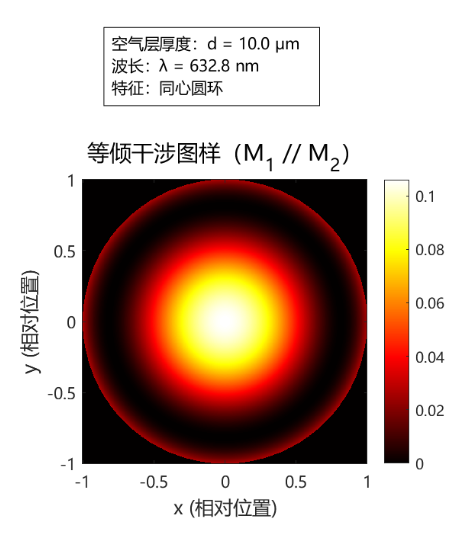
\includegraphics[width=0.6\textwidth]{assets/图3_等倾干涉模拟.png}
\caption{等倾干涉图样模拟（$M_1 \parallel M_2$）}
\label{fig:equal_incline}
\end{figure}

\subsection{等厚干涉模拟}

当动镜 $M_1$ 与虚像 $M_2'$ 之间存在微小夹角 $\alpha$ 时，形成楔形空气层，空气层厚度沿某一方向线性变化。在垂直入射的条件下，光程差仅取决于该点处的厚度 $d(x) = d_0 + \alpha x$。厚度相同的位置对应相同的干涉级次，因而形成一系列平行于楔形交线的直条纹。

模拟中设初始厚度 $d_0 = 10$ $\mu$m，楔角 $\alpha = 5 \times 10^{-4}$ rad。得到的光强分布如图~\ref{fig:equal_thick} 所示。左图展示了规则的平行直条纹，条纹取向垂直于厚度变化的方向；右图的三维视图更清晰地显示了光强沿楔形方向的周期性变化。这一结果与实验中观察到的等厚干涉图样高度吻合。

\begin{figure}[H]
\centering
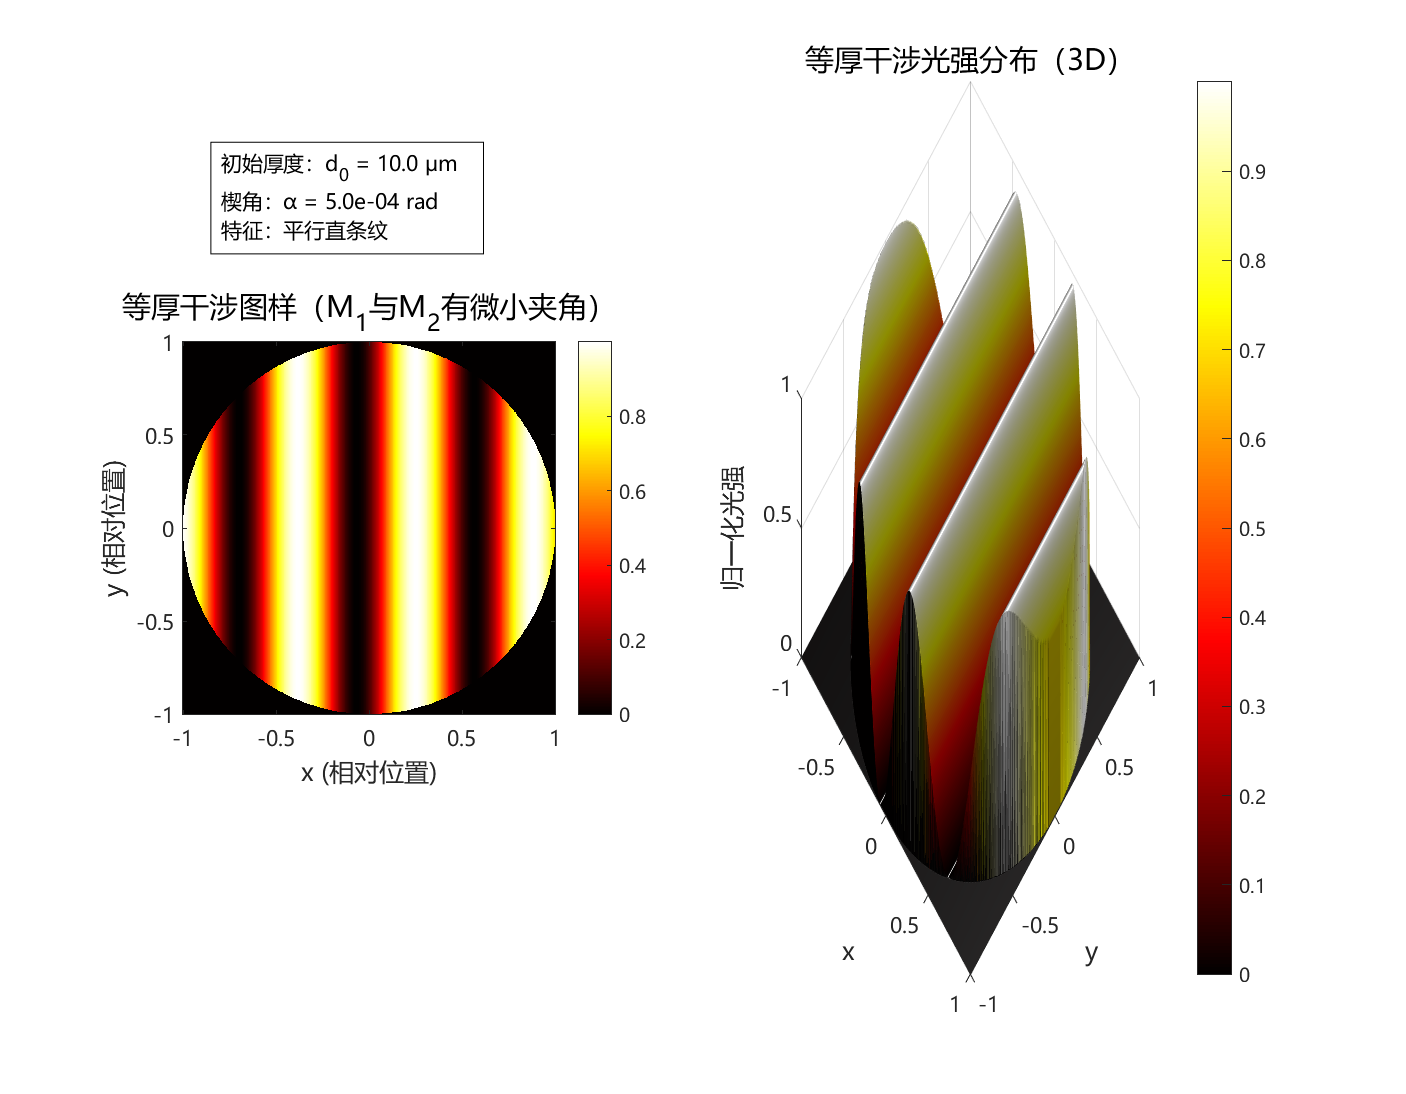
\includegraphics[width=0.9\textwidth]{assets/图4_等厚干涉模拟.png}
\caption{等厚干涉图样模拟（$M_1$ 与 $M_2$ 有微小夹角）}
\label{fig:equal_thick}
\end{figure}

\subsection{两种干涉类型的对比}

图~\ref{fig:comparison} 将等倾干涉和等厚干涉的模拟结果并列展示，清晰地对比了两种干涉类型的图样特征。等倾干涉产生同心圆环，反映了光程差随入射角的变化；等厚干涉产生平行直条纹，反映了光程差随空间位置（厚度）的变化。两种干涉类型的物理本质相同，都是由两束相干光叠加产生，但由于几何条件不同而呈现出不同的图样形态。

\begin{figure}[H]
\centering
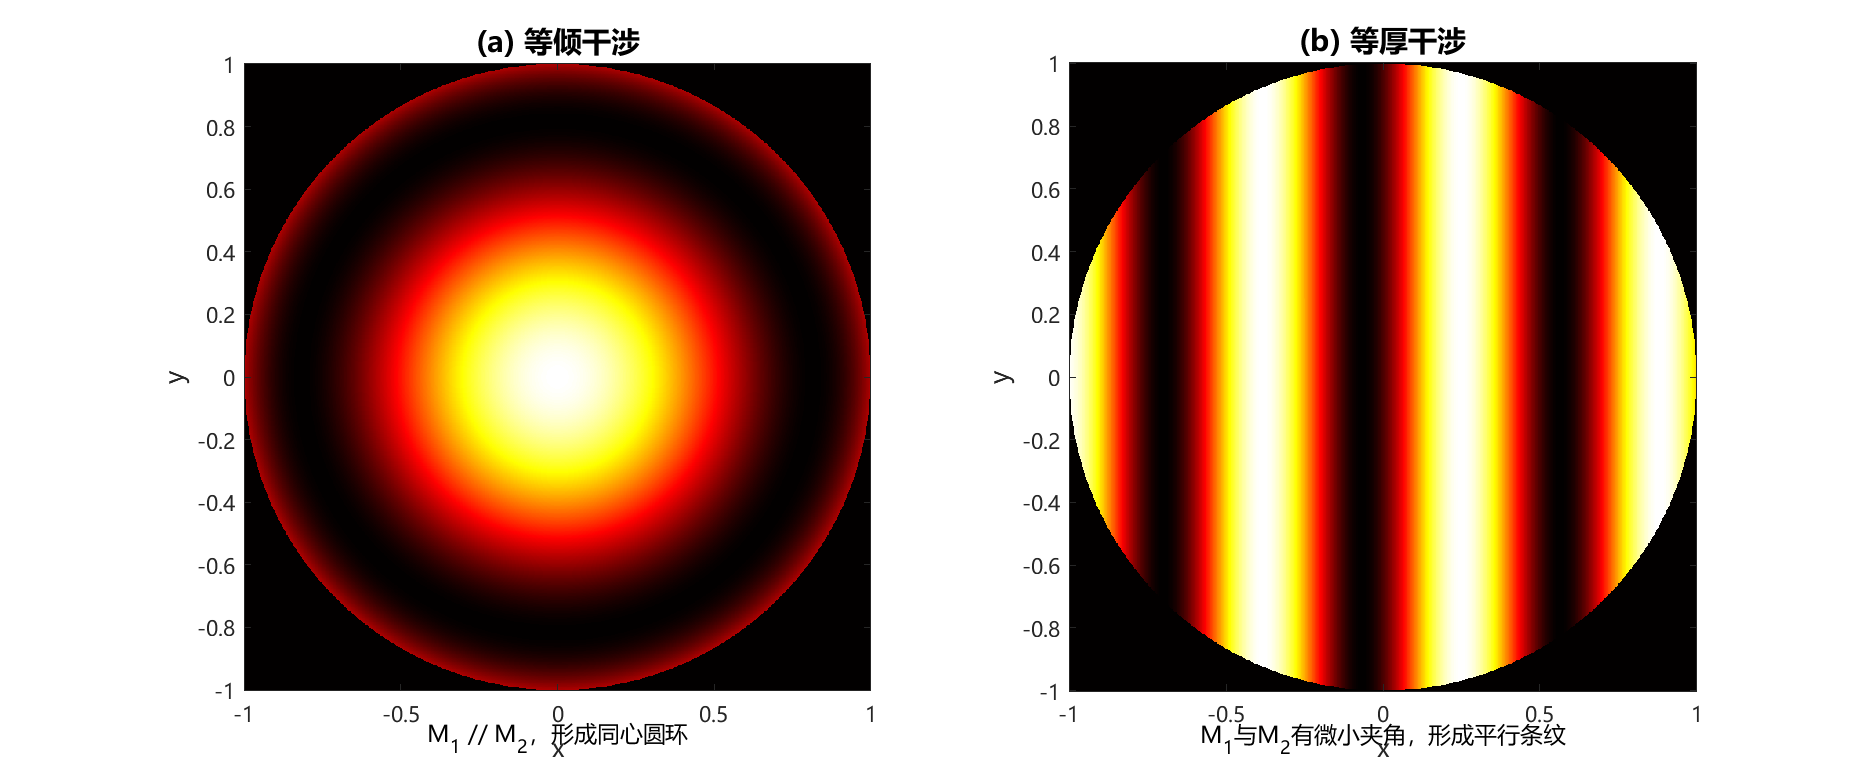
\includegraphics[width=0.95\textwidth]{assets/图5_干涉类型对比.png}
\caption{等倾干涉与等厚干涉图样对比}
\label{fig:comparison}
\end{figure}

通过模拟分析可以更深入地理解干涉条纹的形成机制，并为实验调节和观察提供理论指导。在实际实验中，通过微调反射镜的倾斜程度，可以在两种干涉类型之间连续过渡，甚至观察到两者的混合图样。

\section{误差分析}

本实验测得的光波波长为 626.27 nm，与 He-Ne 激光的标准波长 632.8 nm 相比，相对误差为 1.03\%。这一结果精度较高，但仍存在一定偏差。误差的主要来源可归纳为以下几个方面。

\textbf{测微螺旋的读数误差}是最直接的误差来源。测微螺旋的最小读数为 0.01 mm，读数时存在估读误差，通常在半个分度值以内，即约 $\pm 0.005$ mm。此外，螺旋机构本身可能存在回程差和螺距不均匀性，尤其在长时间使用或维护不当的情况下，这种系统性偏差会更加明显。为了减小回程差的影响，本实验始终保持同一旋转方向进行测量。

\textbf{条纹计数误差}同样不可忽视。在观察干涉条纹移动时，条纹从中心涌出或缩入的速度受旋转速度的影响。如果旋转过快，条纹变化迅速，容易造成漏数或重复计数。此外，当条纹中心不在视场正中时,判断条纹是否完全通过中心也会带来一定的主观性。本实验采用每 50 个条纹记录一次读数的方法，虽然可以通过多次测量平均来减小随机误差，但每次计数的累积误差仍会对最终结果产生影响。

\textbf{干涉条纹的清晰度和稳定性}受到多种因素影响。空气扰动、温度变化和机械振动都会导致光程差发生微小波动，使条纹模糊或抖动,增加计数和读数的困难。实验环境的稳定性对测量精度有重要影响。此外，激光束的准直性和扩束镜的质量也会影响干涉条纹的对比度和清晰度。

\textbf{仪器调整的精度}直接决定了干涉条纹的质量。如果两束反射光不能很好地重合，或者动镜与定镜的平行度不够理想，条纹会变得模糊或畸变，从而影响计数的准确性。尽管在实验开始前进行了细致调节，但受限于人眼的分辨能力和微调螺钉的灵敏度，不可能达到绝对理想的状态。

\textbf{数据处理中的模型假设}也可能引入误差。线性拟合假设位移与条纹数严格成正比，但在实际情况下，测微螺旋的螺距可能存在微小的非线性,或者在不同测量区间内有所差异。虽然拟合的决定系数 $R^2 = 0.999097$ 表明线性模型整体适用性很好,但仍有微小的偏离。

综合上述误差来源，本实验的不确定度主要由测微螺旋的读数精度和条纹计数的累积误差决定。通过线性拟合方法综合利用所有数据点，可以有效降低随机误差的影响,得到的波长不确定度约为 6.0 nm，相对不确定度约为 1\%。这一精度水平对于教学实验而言是令人满意的，充分展示了迈克尔逊干涉仪在精密测量中的优越性能。

若要进一步提高测量精度，可以采取以下改进措施：使用精度更高的测微装置或光学编码器；在恒温、隔振的环境中进行实验；采用光电探测器代替人眼计数条纹；增加测量次数并对数据进行更精细的统计分析；对测微螺旋进行标定,修正系统性偏差等。

\section{实验结论}

通过本次迈克尔逊干涉仪测量光波波长实验，成功观察了等倾干涉和等厚干涉两种干涉现象，深入理解了干涉条纹的形成机制和物理本质。主要结论如下：

\textbf{1. 验证了迈克尔逊干涉仪的工作原理}

实验过程中观察到的同心圆环（等倾干涉）和平行直条纹（等厚干涉）与理论预期完全一致。通过调节反射镜的相对位置,可以在两种干涉类型之间自由切换,充分体现了分振幅干涉的基本特征。数值模拟的结果与实验观察高度吻合，进一步验证了理论分析的正确性。

\textbf{2. 精确测定了光波波长}

利用干涉条纹的移动测量光波波长，实验测得 He-Ne 激光波长为 $(626.3 \pm 6.0)$ nm，与标准值 632.8 nm 相比,相对误差仅为 1.03\%。动镜位移与干涉条纹数之间的线性关系得到很好验证，拟合的决定系数 $R^2 = 0.999097$，表明实验数据具有高度的系统性和重现性。

\textbf{3. 掌握了精密光学测量方法}

通过本实验,掌握了迈克尔逊干涉仪的调节技巧，包括光路对准、反射镜平行度调节、干涉条纹优化等关键步骤。学习了利用线性拟合处理实验数据的方法,以及如何通过残差分析和不确定度评估来检验实验结果的可靠性。这些方法和技能在精密测量和科学研究中具有广泛的应用价值。

\textbf{4. 认识了迈克尔逊干涉仪的重要应用}

迈克尔逊干涉仪不仅是测量光波波长的精密仪器，还在许多基础物理实验和工程应用中发挥重要作用。历史上著名的迈克尔逊-莫雷实验利用该仪器否定了以太的存在，为狭义相对论的建立奠定了实验基础。在现代科技中，基于迈克尔逊干涉原理的激光干涉仪被广泛用于长度标准、微小位移测量、光谱分析、引力波探测等领域，如 LIGO 引力波天文台就采用了长臂迈克尔逊干涉仪来探测时空的微小扰动。

综上所述,本次实验圆满完成了预定目标，通过系统的观察、测量和分析，验证了光的波动性和干涉理论,测定了光波的重要参数，加深了对光学干涉现象的理解，为进一步学习和研究光学奠定了坚实的实验基础。

\clearpage
\appendix

\section{数据处理MATLAB代码}

\subsection{波长测量数据处理}

\begin{lstlisting}[style=Matlab-boxed,caption={迈克尔逊干涉仪数据处理代码}]
%% 迈克尔逊干涉仪实验 —— 数据处理与可视化

clear; clc; close all;
try
    set(0,'DefaultAxesFontName','Microsoft YaHei');
    set(0,'DefaultTextFontName','Microsoft YaHei');
catch
end
if ~strcmp(get(0,'DefaultAxesFontName'),'Microsoft YaHei')
    try
        set(0,'DefaultAxesFontName','SimHei');
        set(0,'DefaultTextFontName','SimHei');
    catch
    end
end
set(0,'DefaultLineLineWidth',1.6);
set(0,'DefaultAxesFontSize',12);

%% ================= 实验数据 =================
% 初始位置（读数）
d0_reading = 5.000;

% 条纹数与对应位置读数
N_fringes = (50:50:600)';
d_position_reading = [6.370; 7.763; 9.405; 11.378; 12.968; 14.482; ...
                      15.979; 17.475; 18.978; 20.538; 22.018; 23.510];
% 读数单位转换系数（每格 = 0.01 mm）
scale_factor = 0.01;

% 计算实际位置（mm）
d0 = d0_reading * scale_factor;
d_position = d_position_reading * scale_factor;

% 计算位移
Delta_d = d_position - d0;

%% ================= 线性拟合 =================
p = polyfit(N_fringes, Delta_d, 1);
k = p(1);  % mm/fringe
b = p(2);

Delta_d_fit = polyval(p, N_fringes);

SS_res = sum((Delta_d - Delta_d_fit).^2);
SS_tot = sum((Delta_d - mean(Delta_d)).^2);
R2 = 1 - SS_res/SS_tot;

%% ================= 波长计算 =================
lambda_nm = 2 * k * 1e6; % nm

lambda_each = 2 * Delta_d ./ N_fringes * 1e6;
lambda_mean = mean(lambda_each);
lambda_std = std(lambda_each, 1);

%% ================= 不确定度分析 =================
n = length(N_fringes);
s = sqrt(SS_res / (n-2));
sx = sqrt(sum((N_fringes - mean(N_fringes)).^2));
u_k = s / sx;
u_lambda = 2 * u_k * 1e6;

%% ================= 结果输出 =================
fprintf('========================================\n');
fprintf('迈克尔逊干涉仪实验数据处理结果\n');
fprintf('========================================\n\n');

fprintf('线性拟合结果：\n');
fprintf('  斜率 k = %.6f mm/条纹\n', k);
fprintf('  截距 b = %.6f mm\n', b);
fprintf('  相关系数 R² = %.6f\n\n', R2);

fprintf('波长测量结果：\n');
fprintf('  从拟合斜率：λ = %.2f nm\n', lambda_nm);
fprintf('  各组平均值：λ = %.2f ± %.2f nm\n', lambda_mean, lambda_std);
fprintf('  波长不确定度：u(λ) = %.2f nm\n\n', u_lambda);

fprintf('理论值对比：\n');
fprintf('  He-Ne激光波长标准值：632.8 nm\n');
fprintf('  相对误差：%.2f%%\n', abs(lambda_nm - 632.8) / 632.8 * 100);
fprintf('========================================\n');

%% ================= 绘图 =================
figure('Name','位移-条纹数关系','Color','w','Position',[100 100 800 600]);
scatter(N_fringes, Delta_d, 60, 'filled', 'MarkerFaceColor', [0.2 0.4 0.8]);
hold on;
xx = linspace(min(N_fringes), max(N_fringes), 200);
plot(xx, polyval(p,xx), '-', 'Color', [0.8 0.2 0.2], 'LineWidth', 2);
grid on; box on;
title('迈克尔逊干涉仪：动镜位移与条纹数的关系');
xlabel('条纹数 N');
ylabel('动镜位移 Δd (mm)');

txt = sprintf('线性拟合：Δd = %.4f × N + %.4f\nR² = %.6f\n\n测得波长：λ = %.2f nm', ...
              k, b, R2, lambda_nm);
text(100, max(Delta_d)*0.85, txt, 'Interpreter','none', ...
     'FontSize', 11, 'BackgroundColor', 'w', 'EdgeColor', 'k');
legend({'实验数据','线性拟合'}, 'Location','southeast');

saveas(gcf, 'assets/图1_位移条纹关系.png');
\end{lstlisting}

\subsection{干涉图样模拟}

\begin{lstlisting}[style=Matlab-boxed,caption={干涉图样模拟代码（节选）}]
%% 迈克尔逊干涉仪 —— 干涉图样模拟

%% 参数设置
lambda = 632.8e-9; % He-Ne激光波长 (m)
d0 = 10e-6;        % 空气层厚度 (m)
N = 800;
x = linspace(-1, 1, N);
y = linspace(-1, 1, N);
[X, Y] = meshgrid(x, y);

%% 等倾干涉
R = sqrt(X.^2 + Y.^2);
theta_max = 0.1;
theta = theta_max * R;
delta_equal_incline = 2 * d0 * cos(theta);
phi_equal_incline = 2 * pi * delta_equal_incline / lambda;
I_equal_incline = cos(phi_equal_incline / 2).^2;
mask = R <= 1;
I_equal_incline = I_equal_incline .* mask;

%% 等厚干涉
alpha = 5e-4;
d_wedge = d0 + alpha * X * 1e-3;
delta_equal_thick = 2 * d_wedge;
phi_equal_thick = 2 * pi * delta_equal_thick / lambda;
I_equal_thick = cos(phi_equal_thick / 2).^2;
I_equal_thick = I_equal_thick .* mask;
\end{lstlisting}

\end{document}

